% -*- root: ../main.tex -*-

%  piano di lavoro adottato. A tal fine, per ogni attività svolta durante la preparazione dell'elaborato (ad esempio: studio di una tecnologia, progettazione di un componente, implementazione di un algoritmo ecc. . . ) deve essere chiarita la collocazione temporale e devono essere indicate le risorse impiegate per svolgerla (giorni/uomo). I candidati possono ricorrere a opportuni diagrammi come quello di Gantt.

\chapter{Piano di lavoro}
Il lavoro è stato svolto utilizzando un approccio Scrum, con sprint periodici, di cui uno iniziale incentrato sullo studio delle tecnologie. Un diagramma di Gantt è stato creato all'inizio del progetto per definirne le tempistiche. Inizialmente una buona dose di tempo è stata impiegata per un design dettagliato, per non incorrere in cambiamenti in corso d'opera. Inoltre, si è prestata attenzione a costruire la relazione e la documentazione passo passo durante il lavoro. Qui di seguito viene riportato lo schema realizzato inizialmente. 
\begin{figure}[H]
    \caption{Gantt Chart Programmato}
    \label{fig:Gantt}
    \centering
    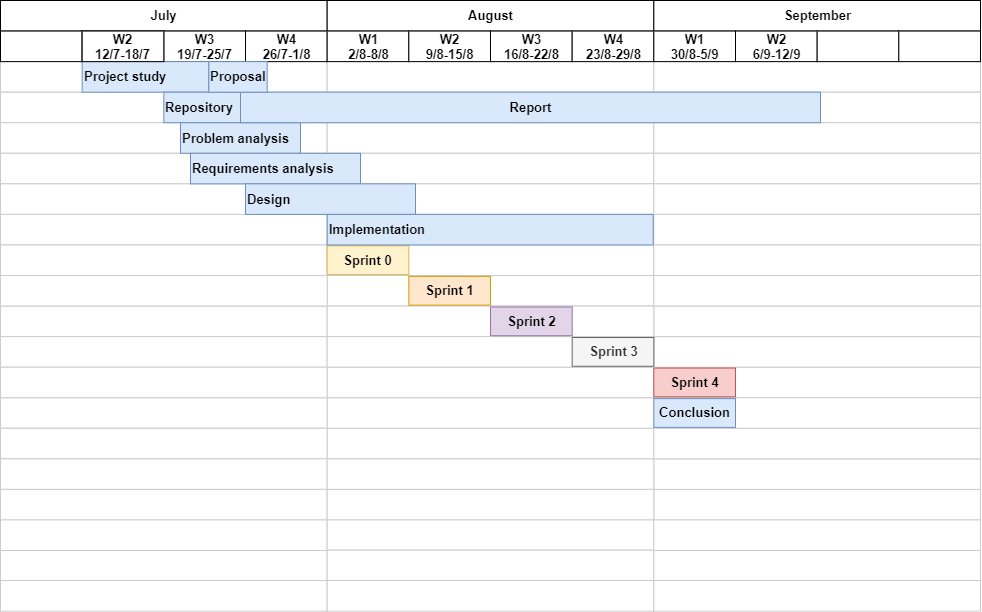
\includegraphics[width=1\textwidth]{DrawIo/GanttChart.png}
\end{figure}

Nonostante il programma dettagliato e le deadlines periodiche il progetto verso la fine si è dilazionato nel tempo. Lo si può vedere chiaramente dalla curva formata dal grafico. Riteniamo però che l'allungamento dei tempi sia dovuto anche a fattori esterni, quali l'inizio delle lezioni e il sovrapporsi di impegni non programmati. Di seguito è riportato il reale andamento del progetto nel tempo. 
\begin{figure}[H]
    \caption{Gantt Chart Effettivo}
    \label{fig:GanttReal}
    \centering
    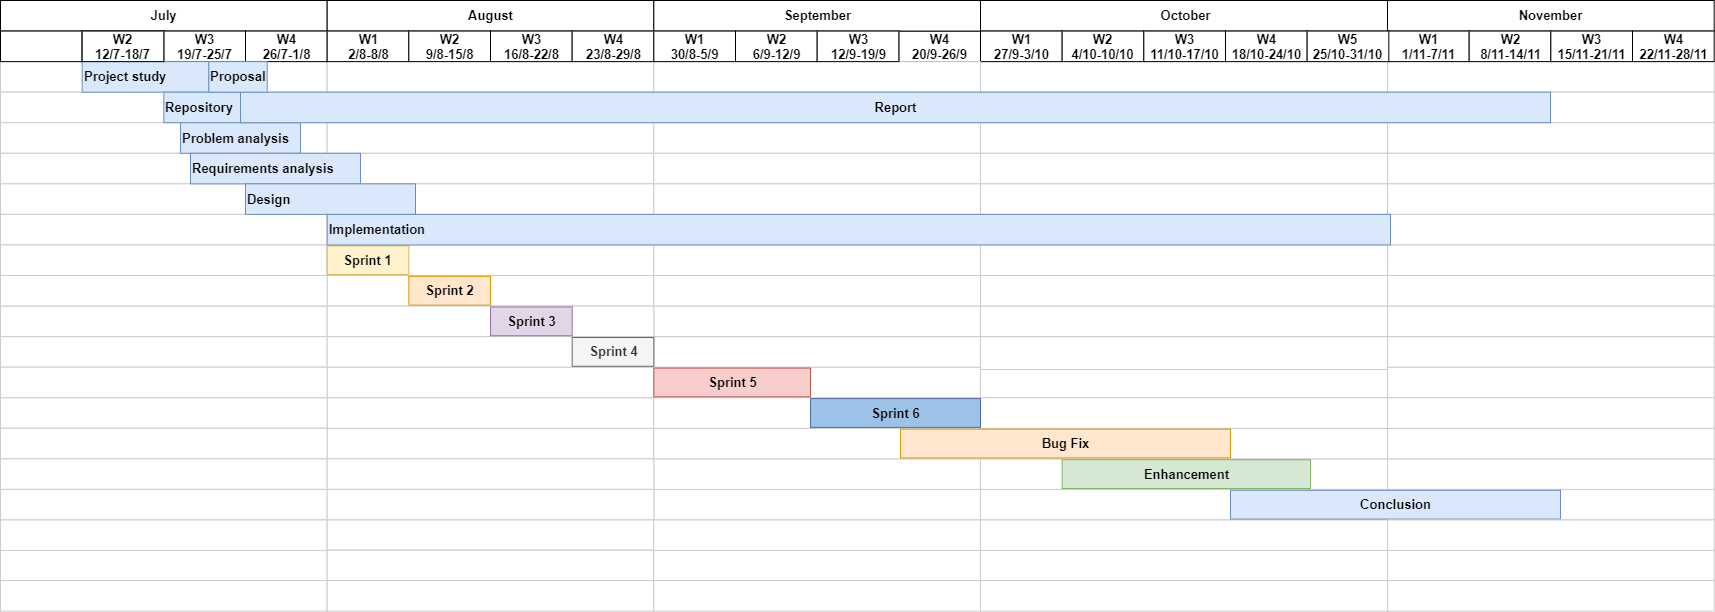
\includegraphics[width=1\textwidth]{DrawIo/GanttChartReal.png}
\end{figure}

\section{Sprints}

\subsection{Svolgimento}
Gli sprint sono stati portati avanti nel seguente modo:
    \paragraph{Sprint Planning}
        Pianificazione a inizio sprint degli obiettivi, tempistiche e responsabilità nel periodo dello sprint corrente. Diviso in due parti:
        \begin{itemize}
        \item\textbf{parte 1} 
            Viene raffinato e rivisto il product backlog, viene effettuata la scelta dello sprint goal (what).
        \item\textbf{parte 2}
            Si decidono gli item e viene raffinato come implementarli (how). Effettuato con solo il team senza la figura del product owner
        \end{itemize}
    \paragraph{[Iterativo] Daily scrum} Breve meeting svolto giornalmente. Viene utilizzato per gli aggiornamenti sull'andamento del progetto, senza scendere nei dettagli implementativi.
    \paragraph{[Occasionale] Pair Programming } Utilizzato per risolvere problemi che causano il blocco di un componente del team per parecchio tempo su una issue.
    \paragraph{Meeting finale}
        Riflessioni e considerazioni finali sullo spint passato. Suggerimenti per migliorare il prossimo. Diviso in tre parti: 
        \begin{itemize}
        \item\textbf{Product backlog refinement} aggiunta di dettagli e riordino del product backlog
        \item\textbf{Sprint review} è stato ispezionato l'incremento, il Minimum Viable Product o di risultati sul processo. Discernere cosa è stato fatto e cosa no.
        \item\textbf{Retrospettiva} Considerazioni sul team stesso e sui miglioramenti per il prossimo sprint. 
        \end{itemize}
        
        

\subsection{Sprint 0}
All'interno dello  \href{https://github.com/orgs/Weather-Vortex/projects/2}{sprint 0} il focus è stato posto sull'apprendimento delle tecnologie scelte più dal punto di vista tecnico. Inoltre è stato impostato l'ambiente di sviluppo, rendendolo condiviso e unificato. 
Infine sono state definite le operazioni chiave per le API REST, lo user data model e le procedure di user authentication, login e register.
\paragraph{Deliverables} 
\begin{itemize}
    \item architettura base server
    \item scheletro relazione
\end{itemize}


\subsection{Sprint 1}
All'interno dello  \href{https://github.com/orgs/Weather-Vortex/projects/3}{sprint 1} il focus è stato sulla creazione del client, con l'utilizzo di Vue per creare le pagine base di esso e alcuni componenti chiave.
\paragraph{Deliverables} 
\begin{itemize}
    \item Pagina 404
    \item Pagina About
    \item Menu
\end{itemize}

\subsection{Sprint 2}
All'interno dello  \href{https://github.com/orgs/Weather-Vortex/projects/4}{sprint 2} sono stati fatti cambiamenti e miglioramenti su più parti del sito. Arrivati a questo punto inoltre è stato necessario anche occuparsi di bug creati in precedenza. E' stato aggiunto il deploy automatico su GH Pages. Nuovi campi centralina sono stati aggiunti. La geolocalizzaizone ora acquisisce la posizione corrente. 
\paragraph{Deliverables} 
\begin{itemize}
    \item Forecast Page
    \item Homepage
    \item Responsiveness Fixed
    \item Footer
\end{itemize}

\subsection{Sprint 3}
All'interno dello  \href{https://github.com/orgs/Weather-Vortex/projects/5}{sprint 3} il focus è stato sul creare i componenti principali rimanenti. La pagina dei feedback è stata modellata dal lato grafico. L'homepage è stata completata assieme alla pagina di autenticazione. Sono stati aggiunti per gli sviluppatori dei codici rappresentanti le varie condizioni meteo. 
\paragraph{Deliverables} 
\begin{itemize}
    \item Homepage completa
    \item Leave Feedback Page
    \item Autentication Page
\end{itemize}

\subsection{Sprint 4}
All'interno dello  \href{https://github.com/orgs/Weather-Vortex/projects/6}{sprint 4} il focus è stato nuovamente sulla correzione di errori e bug. Le routes sono state inoltre rifattorizzate. Sono stati aggiunti gli alert per rendere più intuitiva la navigazione del sito. 
\paragraph{Deliverables} 
\begin{itemize}
    \item Refactoring 
    \item Bug fix
    \item Alert
\end{itemize}

\subsection{Sprint 5}
All'interno dello  \href{https://github.com/orgs/Weather-Vortex/projects/7}{sprint 5} la mole di lavoro è stata notevole, essendo lo sprint finale. I feedback degli utenti sono stati recuperati dal DB e mostrati. La route per la password dimenticata è stata completata.
Inoltre sono state implementate le previsioni meteo dalle stazioni. La funzionalità dell'aggregazione delle previsioni è stata definita. 
\paragraph{Deliverables} 
\begin{itemize}
    \item Feedback Page 
    \item Forgot Password
    \item IoT Forecast
    \item Aggregation Forecasts
\end{itemize}

